\chapter{Implementation}
In this chapter, the steps involved in turning a theoretical design into a tangible system will be outlined. Since the synthesis chapter dealt with an explanation of the functions of each module and simulations, with a subsequent evaluation of the outcomes, this chapter will focus on the creation of physical hardware setups and reproducing the desired results using lab experiments. As such, each module will be tested independently to validate its function before a larger, more comprehensive experiment is conducted. All figures in this chapter show measurements performed on physical hardware.
\section{Control System}
\begin{figure}[htbp]
	\centering
	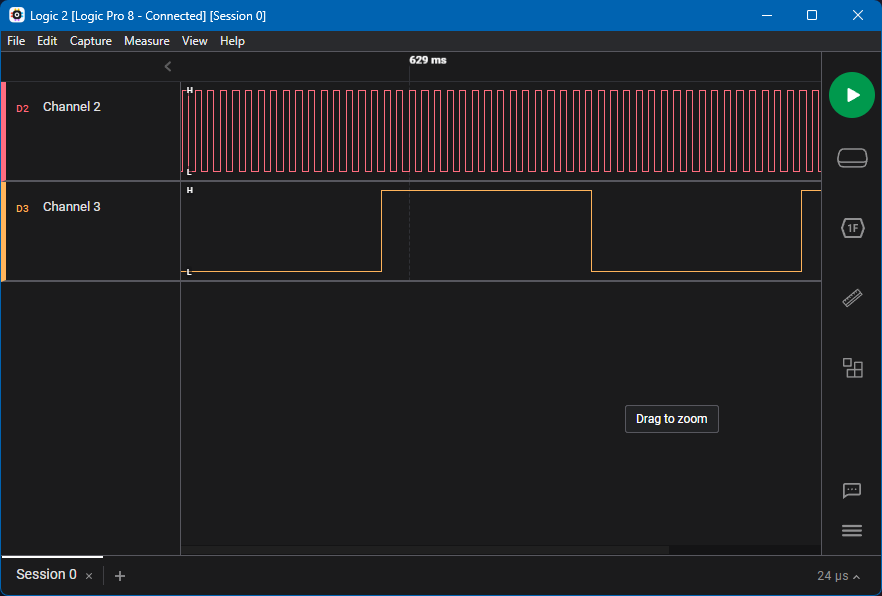
\includegraphics[width=.8\textwidth]{Figures/4_controlsystem_stm32_zephyr.png}
	\caption{STM32 Zephyr RTOS pulser output}
	\label{fig:4_stm32_zephyr_pulser}
\end{figure}
During the initial implementation stage of the control system, a bring-up of the STM32F411RE board and several pulse signals were succesfully generated. In \cref{fig:4_stm32_zephyr_pulser}, two pulse signals can be seen. In Channel 2, \qty{5}{\mega\hertz} ultrasound pulse can be seen. In Channel 3, the \qty{10}{\kilo\hertz} PRF signal can be seen. Unfortunately, soon thereafter it was discovered a limitation of the API in Zephyr is not mature enough developed for power systems such as the half-bridge in the transmitter circuit. In more practical terms, it was not possible to generate two complementary signals with dead-time using the existing Zephyr PWM API. To continue with that solution, a new PWM driver would have to be written from scratch, which is no trivial task. Alternative solutions were investigated. Another option was to use the \gls{hal} provided by the manufacturer of the microcontroller, but this would also mean an increased amount of development time for the control system since the \gls{hal} is rudimentary in implementation and has little abstraction. However, it was decided to try an alternative system known as PYNQ Z1, which is a development board by Agilent. On the PYNQ Z1 board is a Zynq 7000 \gls{soc}. Inside the Zynq 7000 SoC there are both an \gls{fpga} and Arm based processor. PYNQ is an open-source framework that runs on Xilinx compute platforms where higher levels of abstraction enable faster productivity.

\begin{figure}[htbp]
	\centering
	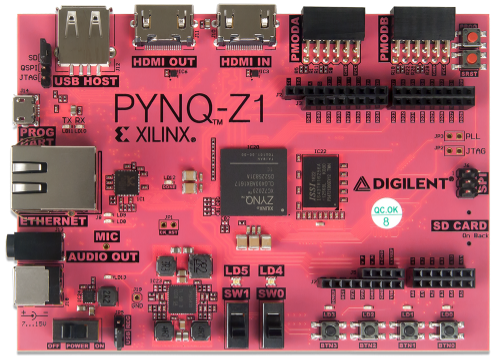
\includegraphics[width=.8\textwidth]{Figures/4_pynq_z1_pcb_pic.png}
	\caption{PYNQ-Z1 development board}
	\label{fig:4_controlsystem_pynq_z1_pcb}
\end{figure}

Seen in \cref{fig:4_controlsystem_pynq_z1_pcb} is the development board with its peripherals. The development of a prototype pulser system will be done by implementating an FPGA project in Vivado and then generating the \gls{bitstream}. After this, the FPGA artifacts are generated as a \texttt{.bit} and \texttt{.hwh} file. These two files are used in the JupyterLab environment as an overlay to configure the logic of the FPGA and output signals on the PMOD-A connector.

\begin{figure}[htbp]
	\centering
	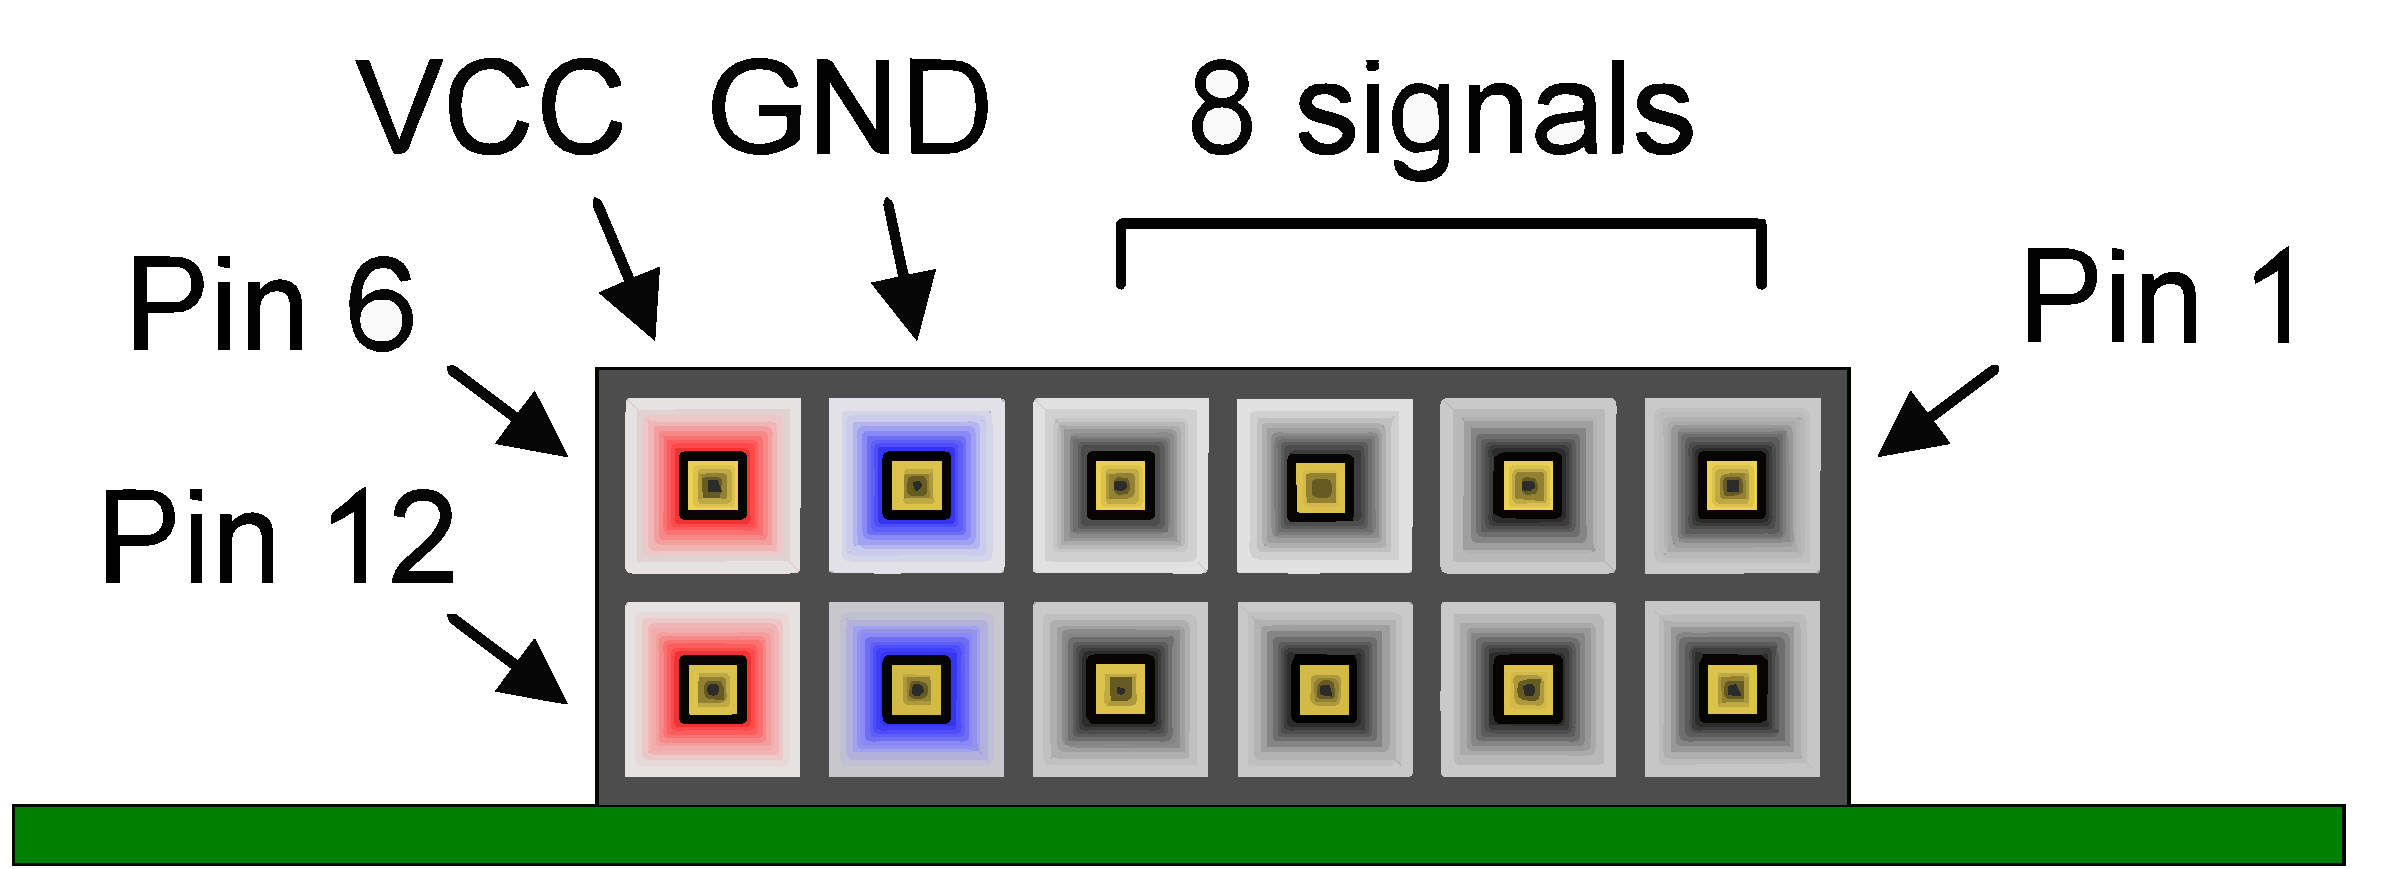
\includegraphics[width=.8\textwidth]{Figures/4_pynq-z1-pmod.pdf}
	\caption[PYNQ Z1 PMOD port diagram]{PYNQ Z1 PMOD port diagram \cite{pynqrm}}
	\label{fig:4_controlsystem_pynq_z1_pmod}
\end{figure}

On the PYNQ-Z1 board, the PMOD ports are 12-pin female connectors with 0.1 inch spacing that connect to normal 12-pin headers. As illustrated in \cref{fig:4_controlsystem_pynq_z1_pmod}, each 12-pin PMOD port offers two 3.3V VCC signals (pins 6 and 12), two GND signals (pins 5 and 11), and eight logic signals. Each PMOD port on a PYNQ board is classified as normal, MIO linked, XADC, or high-speed. The PYNQ-Z1 features two PMOD ports, both of which are high-speed. For maximal switching rates, the High-speed PMOD ports route their data signals as impedance matched differential pairs. For further protection, they feature pads for loading resistors, however the PYNQ-Z1 ships with these loaded as 0-Ohm shunts. With the series resistors shunted, these PMOD ports provide no short-circuit protection but allow for substantially quicker switching rates. Pins 1 and 2, pins 3 and 4, pins 7 and 8, and pins 9 and 10 are coupled to neighboring signals in the same row. Traces are routed in a \qty{100}{\ohm} ($\pm\qty{10}{\percent}$) differential configuration. Coupled pairs may produce crosstalk if pins on this port are utilized as single-ended signals. Because it is being used as a single-ended signal in this application, one of the pins is grounded and its pair is utilized for the single-ended signal. Because the High-Speed PMOD ports employ \qty{0}{\ohm} shunts instead of protection resistors, the user must exercise caution to avoid shorts.

\begin{listing}[htbp]
	\caption{Constraints on Pulse Generator and Control System}
	\label{lst:4_controlsystem_constraints}
	\begin{mintedvhdl}
set_property IOSTANDARD LVCMOS33 [get_ports PULSE]
set_property IOSTANDARD LVCMOS33 [get_ports PWM]
set_property IOSTANDARD LVCMOS33 [get_ports PWMN]
set_property IOSTANDARD LVCMOS33 [get_ports GATE]
set_property IOSTANDARD LVCMOS33 [get_ports PRF]
set_property IOSTANDARD LVCMOS33 [get_ports CLK]
set_property PACKAGE_PIN Y16 [get_ports PULSE]
set_property PACKAGE_PIN Y18 [get_ports PWM]
set_property PACKAGE_PIN Y19 [get_ports PWMN]
set_property PACKAGE_PIN Y17 [get_ports GATE]
set_property PACKAGE_PIN U18 [get_ports PRF]
set_property PACKAGE_PIN U19 [get_ports CLK]

set_property IOSTANDARD LVCMOS33 [get_ports {LEDs[3]}]
set_property IOSTANDARD LVCMOS33 [get_ports {LEDs[2]}]
set_property IOSTANDARD LVCMOS33 [get_ports {LEDs[1]}]
set_property IOSTANDARD LVCMOS33 [get_ports {LEDs[0]}]
set_property PACKAGE_PIN R14 [get_ports {LEDs[0]}]
set_property PACKAGE_PIN P14 [get_ports {LEDs[1]}]
set_property PACKAGE_PIN N16 [get_ports {LEDs[2]}]
set_property PACKAGE_PIN M14 [get_ports {LEDs[3]}]
	\end{mintedvhdl}
\end{listing}

When programming an FPGA with software like as Xilinx's Vivado, it becomes necessary to inform the system which physical pins on the FPGA correspond to the FPGA ports defined in the VHDL code. This is quite similar to putting a register high or low on a microcontroller to turn an LED on or off, operate a clock, or function as a data line. However, with a microcontroller, many of these pins are \enquote{hard-wired} in the sense that they cannot be relocated to a physically different pin on the microcontroller. In general, it's just not an option. This is not the case with an FPGA; instead, the hardware interface is established in VHDL and then the appropriate inputs and outputs on that interface are constrained to whichever pins on the FPGA are required, making FPGAs incredibly versatile for complicated and bespoke designs. In \cref{lst:4_controlsystem_constraints}, the constraints can be seen setting the port names to a certain \texttt{IOSTANDARD} and voltage level and the pin name \texttt{PACKAGE\_PIN}. All the described pins are \gls{io} available on the PMOD port of the PYNQ-Z1.

\begin{figure}[htbp]
	\centering
	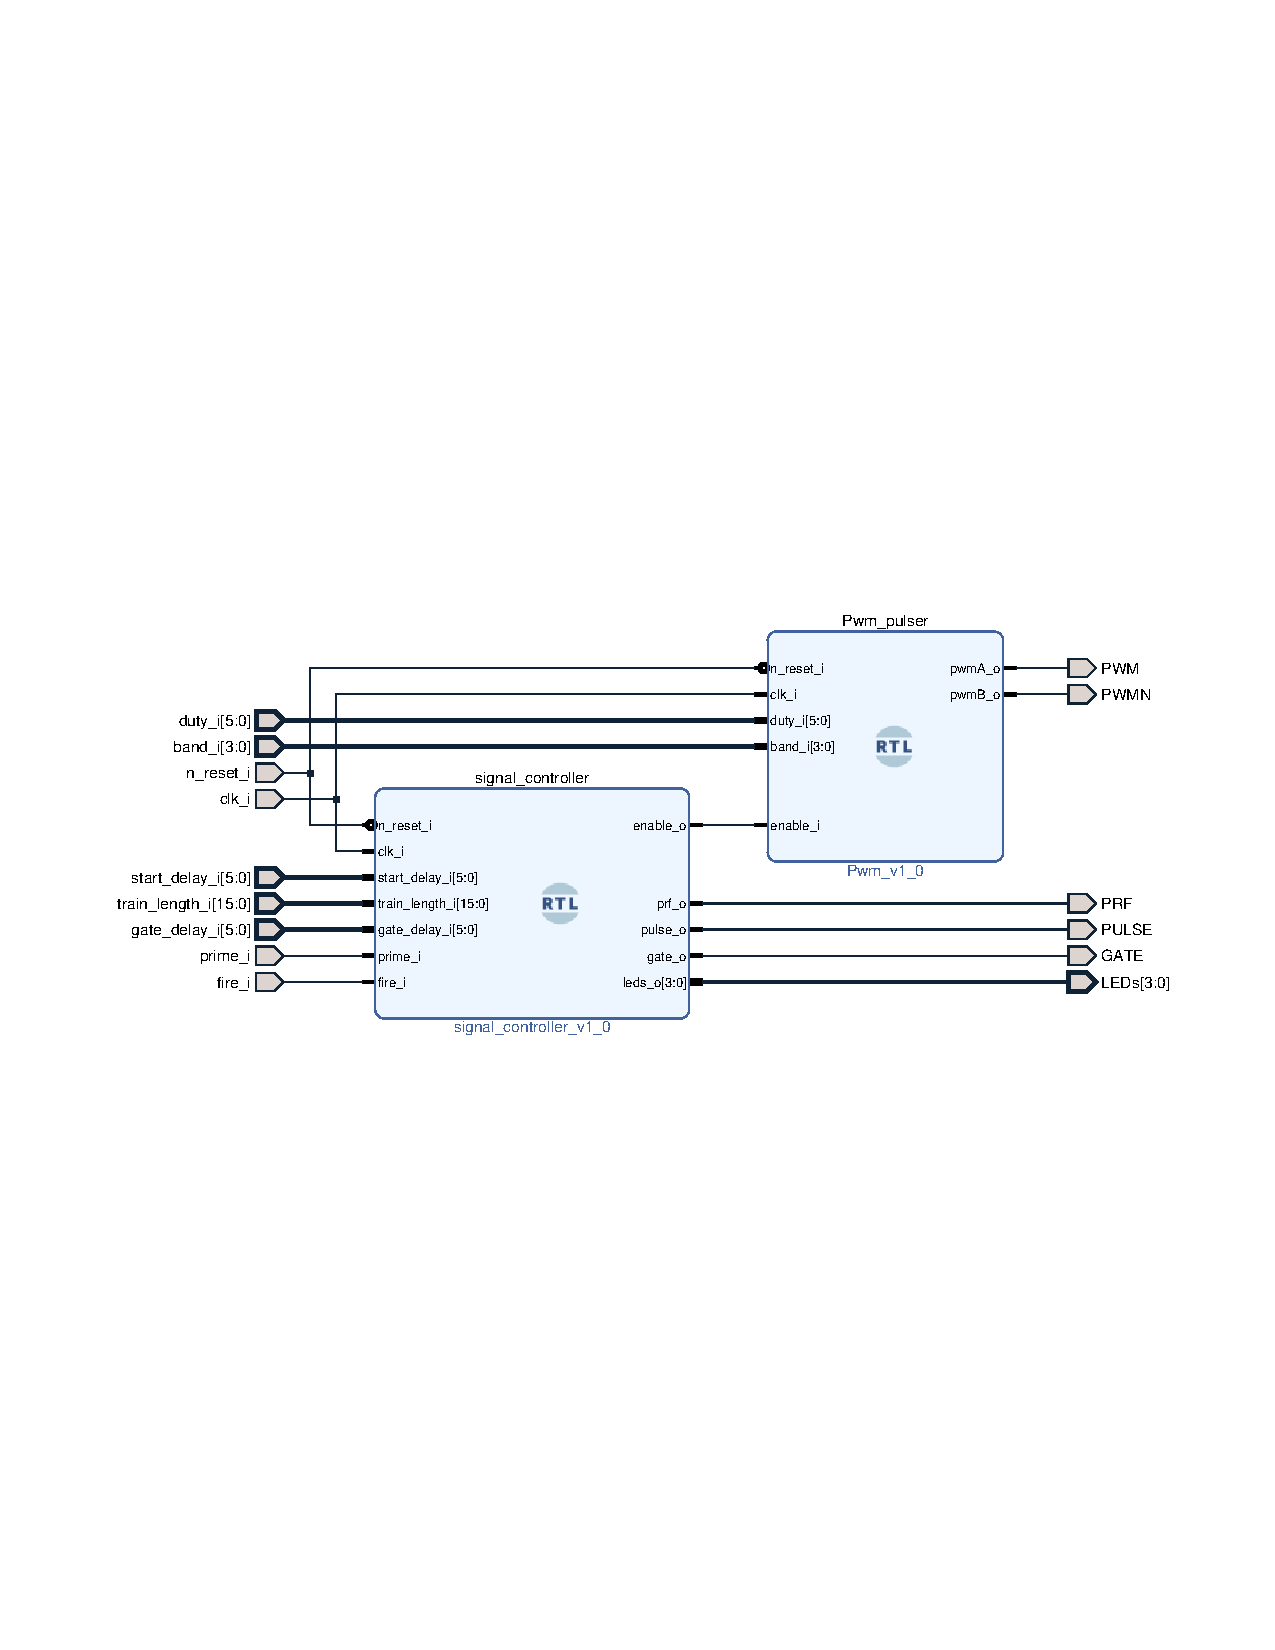
\includegraphics[width=.8\linewidth]{Figures/4_controlsystem_pulser.pdf}
	\caption{PWM pulser and signal controller as a block diagram with inputs and outputs}
	\label{fig:4_controlsystem_pulser}
\end{figure}

\begin{figure}[htbp]
	\centering
	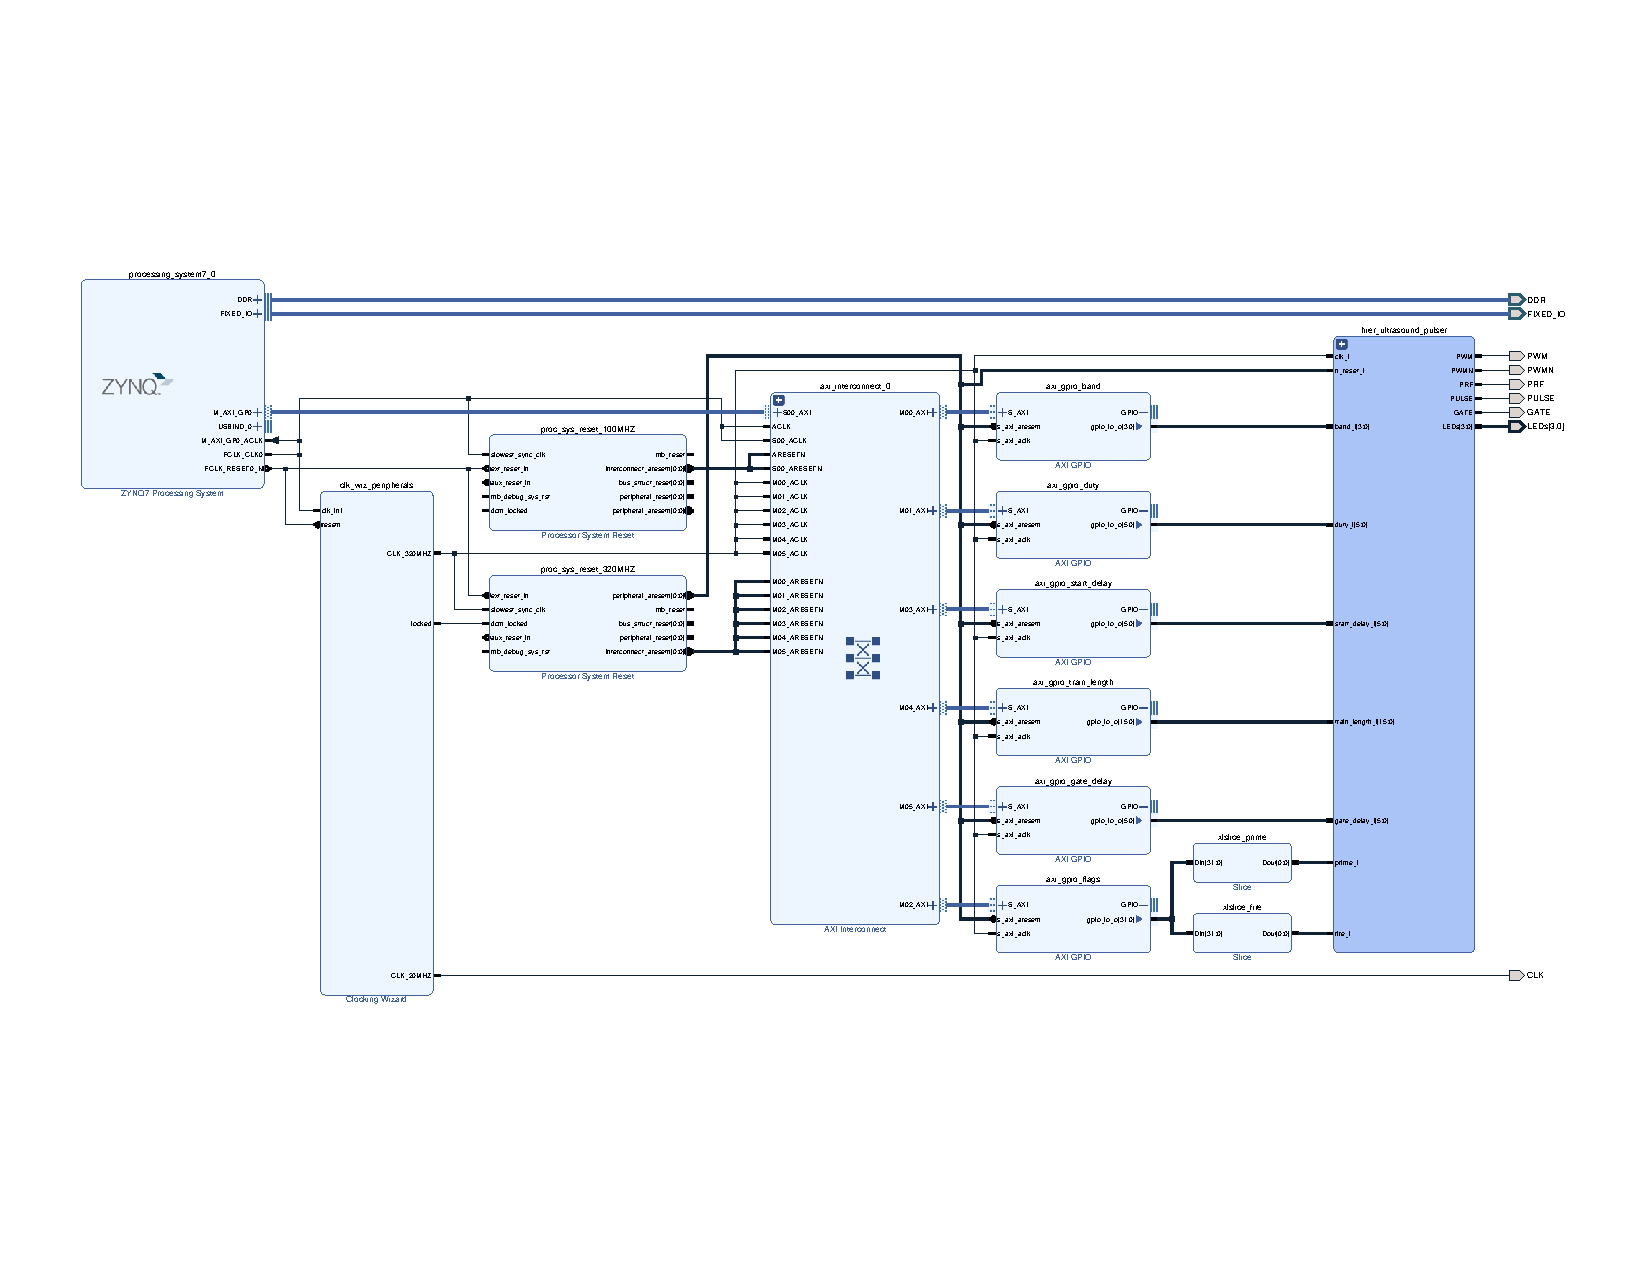
\includegraphics[width=\linewidth]{Figures/4_controlsystem_top_bd.pdf}
	\caption{Top level block diagram of the FPGA overlay with AXI interconnects and registers}
	\label{fig:4_controlsystem_top_bd}
\end{figure}

\section{Power Stage}
\begin{figure}[htbp]
	\centering
	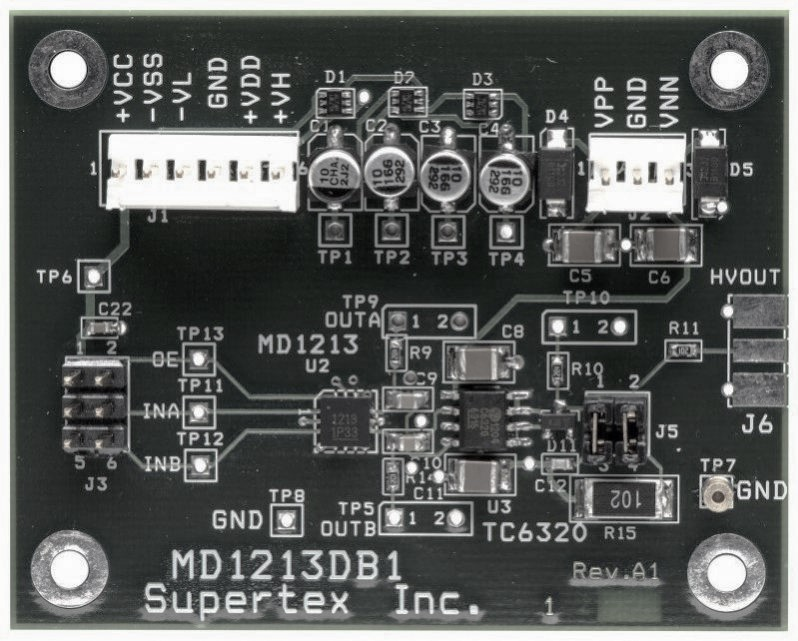
\includegraphics[width=.8\textwidth]{Figures/4_transmitter_pcb_pic.jpg}
	\caption{MD1213DB1 High Speed Pulser}
	\label{fig:4_transmitter_pcb_pic}
\end{figure}
A picture of the power stage PCB can be seen in \cref{fig:4_transmitter_pcb_pic}. An experiment is conducted to validate the function of the power stage. Using the jumpers, the PCB is configured without its onboard load, and a \gls{pzt} transducer is attached with a splitter adapter to connect the other side to an oscilloscope for data acquisition.

\section{Transmit/Receive Switch}
\begin{figure}[htbp]
	\centering
	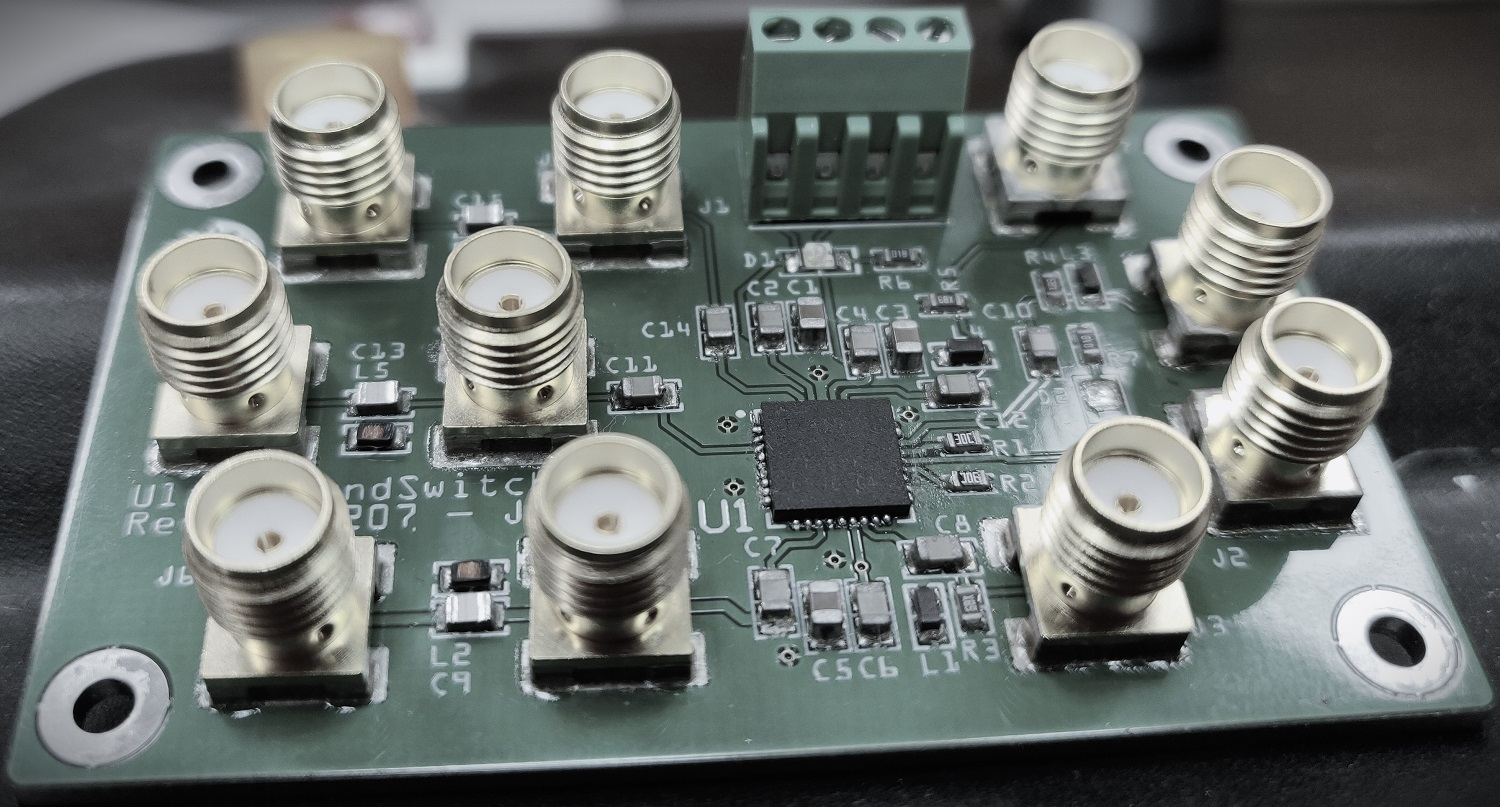
\includegraphics[width=.8\textwidth]{Figures/4_switch_pcb_pic.jpg}
	\caption[Transmit/Receive Switch after assembly]{Transmit/Receive Switch after assembly}
	\label{fig:4_txrx_pcb}
\end{figure}
The entire schematic of the transmit/receive switch can be found in the appendix in \cref{fig:appendix_ultrasoundswitch_a,fig:appendix_ultrasoundswitch_b}. As mentioned in the previous chapter, a PCB layout was made and a batch of 5 was ordered with an accompanying stencil for fast assembly. After the PCBs arrived, the stencil was mounted in the stencil frame and the PCB was aligned for solder paste application. After the solder paste application is completed, all the components are placed on their corresponding footprints and the PCB is placed in the reflow oven. The equipment used in this process is listed in \cref{tab:instruments_solder_work}. The finished assembly can be seen in \cref{fig:4_txrx_pcb}.


\section{Band-Pass Filter}
\begin{figure}[htbp]
	\centering
	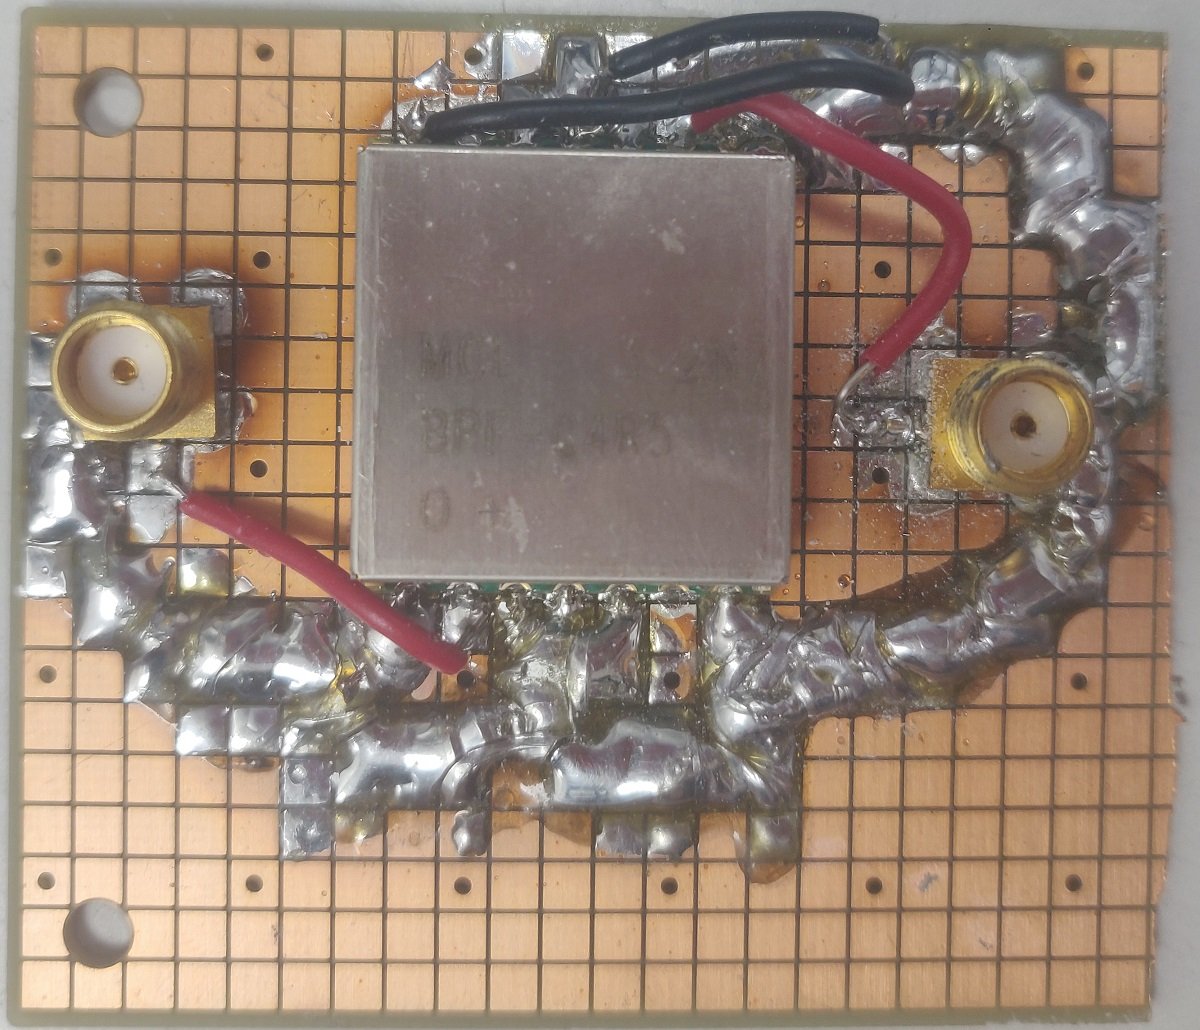
\includegraphics[width=.8\textwidth]{Figures/4_bpf_pcb_pic.jpg}
	\caption{Prototype board of the Band-Pass filter}
	\label{fig:4_bpf_pcb_pic}
\end{figure}
Since the \gls{bp} filter is comprised of a module component in a bespoke form factor, a circuit is implemented on a prototyping board. With the BPF-C4R5+ mounted in the center, input and output connectors are placed on either side with SMA connectors. Since the filter is passive, no power connectors are needed. The prototype board of the \gls{bp} filter can be seen in \cref{fig:4_bpf_pcb_pic}.

\section{Preamplifier}
Before the signal can be demodulated, it must be DC-biased and amplified. This is what the preamplifier is for. For the preamplifier, the circuit is validated using an experiment where a function generator is transmitting a low amplitude sine with ac-coupling and measure the amplified dc-coupled output. Using the AD8332 built-in \gls{lna} and bypassing the \gls{vga} in the circuit, it feeds the amplified output to the next subcircuit Quadrature Demodulator. The preamplifier is part of the same board as the quadrature demodulator in \cref{sec:implementation_demodulator}.

\section{Quadrature Demodulator} \label{sec:implementation_demodulator}
\begin{figure}[htbp]
	\centering
	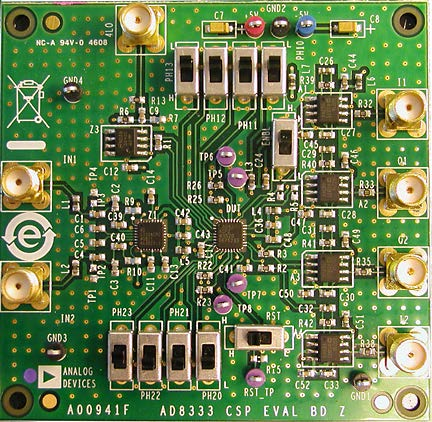
\includegraphics[width=.8\textwidth]{Figures/4_demod_pcb_pic.jpg}
	\caption{Demodulator PCB AD8333-EVALZ}
	\label{fig:4_demod_pcb_pic}
\end{figure}
As described in the previous chapter, the demodulator use an I/Q quadrature demodulation scheme to take two differential RF signals and a quadruple frequency signal, in this case, \qty{5}{\mega\hertz} and \qty{20}{\mega\hertz}, respectively, and determines the frequency difference between the fundamental frequency and the Doppler frequency on the output. After the differential signal from the preamplifier is demodulated, it is output as a current. Next, it is converted using the AD8021 current-to-voltage amplifier coupled with an active \gls{lp} filter to remove the summed demodulated frequency component. What remains are the low-frequency $I$ and $Q$ signals in the \unit{\kilo\hertz} range. The entire schematic of the demodulator can be found in the appendix in \cref{fig:appendix_ad8333}.

\section{Sample and Hold}
\begin{figure}[htbp]
	\centering
	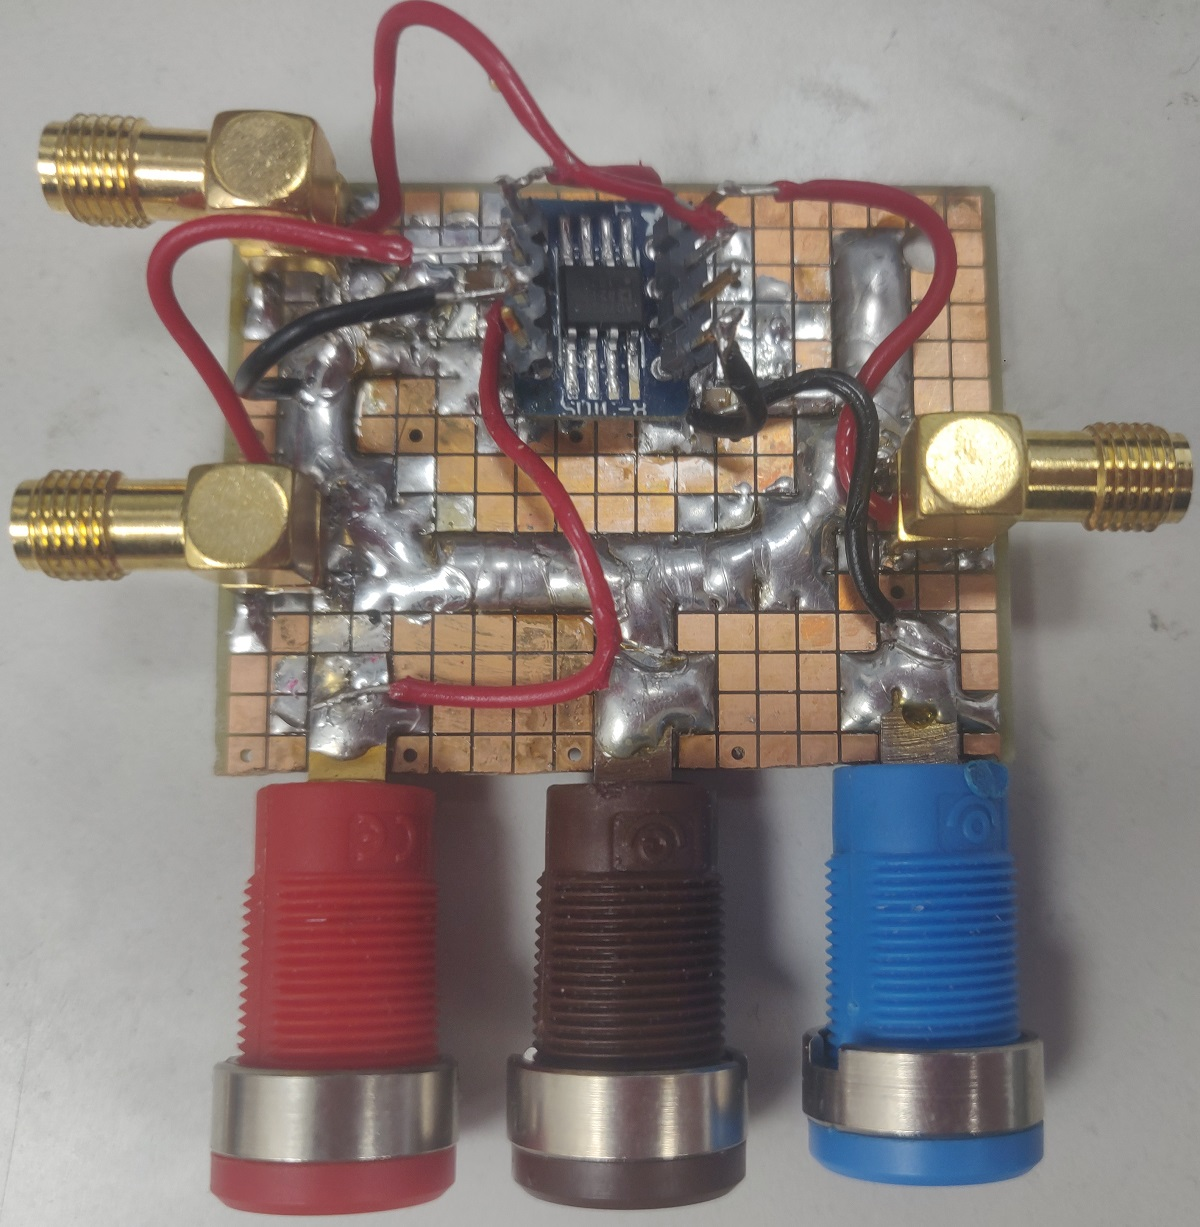
\includegraphics[width=.8\textwidth]{Figures/4_sha_pcb_pic.jpg}
	\caption{Prototype board of the Sample and Hold amplifier}
	\label{fig:4_sha_pcb_pic}
\end{figure}

After each demodulated burst is sampled, between each sample line pulse repetition it is desired to hold the voltage, so the analogue-to-digital conversion that may be running asynchronously does not sample zero-values between the bursts. After the low-frequency signals are output from the quadrature demodulator, they are sampled using the \texttt{GATE} signal output from the control system. This \texttt{GATE} signal is a delayed pulse equal to the length of the pulse train and determines the sampling depth of the \gls{afe}. The prototype board of the sample and hold amplifier can be seen in \cref{fig:4_sha_pcb_pic}.

\section{Active Filter, DC-Coupler}
\begin{figure}[htbp]
	\centering
	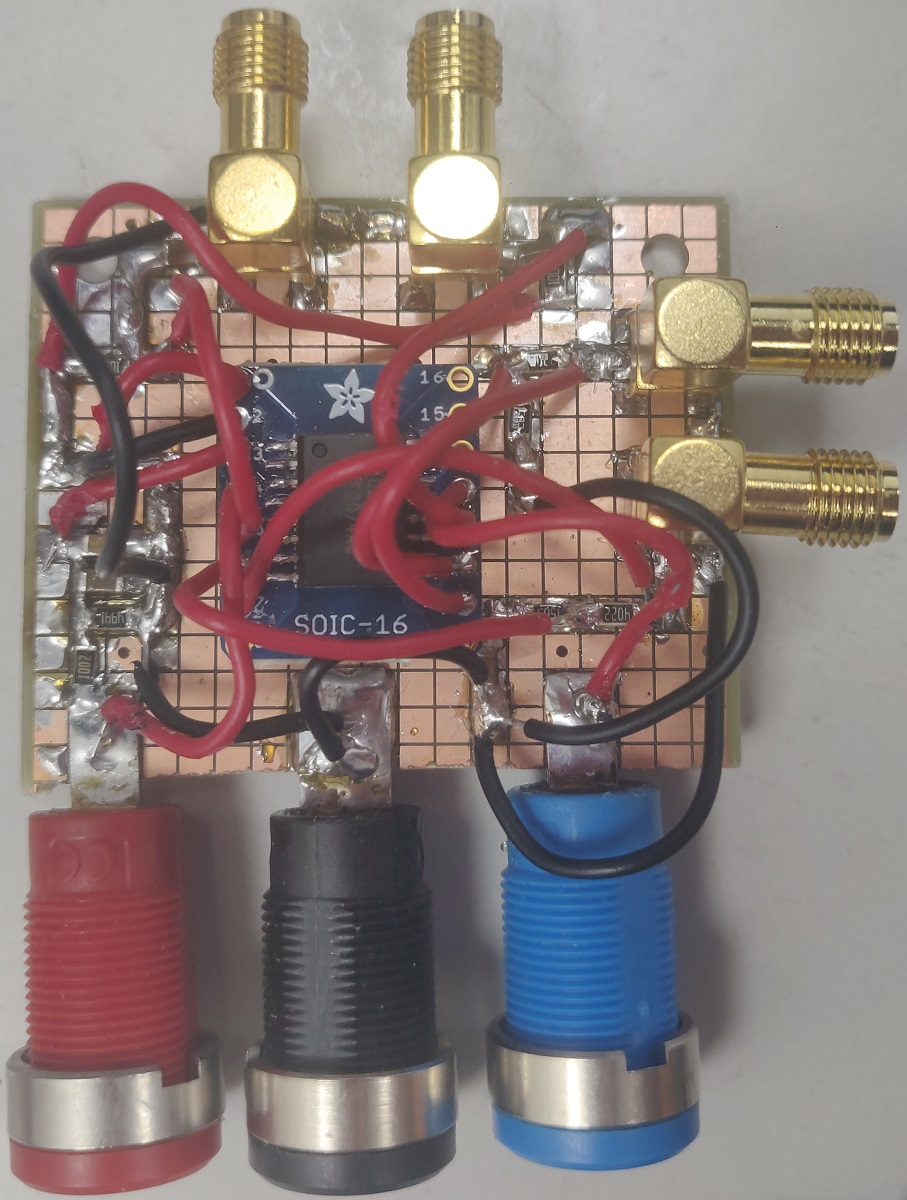
\includegraphics[width=.8\textwidth]{Figures/4_dccoupler_filter_pcb_pic.jpg}
	\caption{Prototype board of the active filter and \gls{dc}-coupler}
	\label{fig:4_dccoupler_pcb_pic}
\end{figure}
Finally, before the signal is digitally quantized by the \gls{adc}, it has to pass through a \gls{hp} filter to remove undesired \gls{prf} or Wall frequency components. The implementation is done on a prototyping board and can be seen in \cref{fig:4_dccoupler_pcb_pic}.

\section{Digital Signal Processor}


%\begin{figure}[H]
%	\centering
%	\begin{circuitikz}[american voltages]
%		\draw
%		(0,0) to [short, *-] (6,0)
%		to [V, l_=$\mathrm{j}{\omega}_m \underline{\psi}^s_R$] (6,2)
%		to [R, l_=$R_R$] (6,4)
%		to [short, i_=$\underline{i}^s_R$] (5,4)
%		(0,0) to [open, v^>=$\underline{u}^s_s$] (0,4)
%		to [short, *- ,i=$\underline{i}^s_s$] (1,4)
%		to [R, l=$R_s$] (3,4)
%		to [L, l=$L_{\sigma}$] (5,4)
%		to [short, i_=$\underline{i}^s_M$] (5,3)
%		to [L, l_=$L_M$] (5,0);
%	\end{circuitikz}
%	\caption{The nodes short, V, R and L are presented here, but there a lot more}
%	\label{fig:circuitikz}
%\end{figure}
%
%\section{Listings (code)}
%
%\Cref{lst:helloworld} is a nicely formatted block of code. A listing will automatically continue on the next page if it encounters a page break. Many different programming languages can be highlighted. Check the \texttt{listings} package documentation for a list of supported programming languages.

%\begin{listing}[htbp]
%\begin{mintedc}
%#include <stdio.h>
%int main()
%{
%	printf("Hello, World!"); /*printf() outputs the quoted string*/
%	if (n == 0 || n == 1){
%		return n;
%	}
%	j = 0;
%	for (i = 0; i < n-1; i++){
%		if (arr[i] != arr[i+1]){
%			arr[j] = arr[i];
%			j++;
%		}
%	}
%	arr[j++] = arr[n-1];
%	return 0;
%}
%\end{mintedc}
%	\caption{Hello world in C}
%	\label{lst:helloworld}
%\end{listing}



